\section{Dominio de Información}

\insertsectionpage

\begin{frame}[allowframebreaks]

  \frametitle{Dominio de Información}

  \begin{columns}
    \begin{column}{.5\textwidth}
      \begin{itemize}
        \item Los datos puestos en contexto generar información.
        \item La información para lograr un fin genera conocimiento.
        \item El conocimiento aplicado a acciones concretas da lugar a sabiduría.
      \end{itemize}
    \end{column}

    \begin{column}{.5\textwidth}
      \begin{figure}[ht]
        \centering
        \includegraphics[width=1\textwidth]{img/Pirámide.png}
        \caption{\label{fig:dominio-piramide} Pirámide del conocimiento.\cite{MinTIC2021}}
      \end{figure}
    \end{column}
  \end{columns}
  
  \begin{figure}[ht]
    \centering
    \includegraphics[width=\textwidth]{img/Pirámide2.png}
    \caption{\label{fig:dominio-piramide-2} Pirámide del conocimiento, ejemplo trivial\cite{MinTIC2021}}
  \end{figure}

\end{frame}

\section{Lineamientos}

\insertsectionpage

\begin{frame}[allowframebreaks]

  \frametitle{Gobierno de la información}

  \begin{columns}
    \begin{column}{.5\textwidth}
      \begin{itemize}
        \item Las entidades públicas deben establecer un modelo de gobierno que regule políticas, responsabilidades, decisiones y métricas para controlar la información.
      \end{itemize}  
    \end{column}

    \begin{column}{.5\textwidth}
      \begin{figure}[ht]
        \centering
        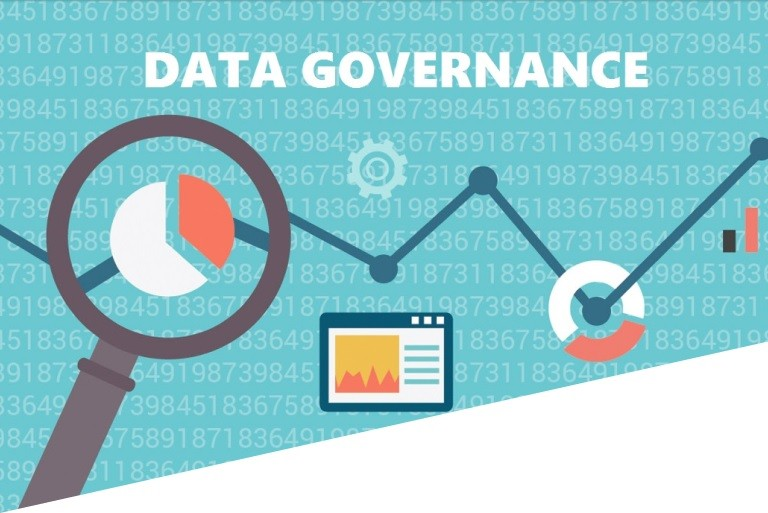
\includegraphics[width=\textwidth]{figures/GobiernoDatos.jpg}
        \caption{Imagen sacada de Bermejo Eduardo\cite{bermejo2023claves}}
      \end{figure}

    \end{column}
  \end{columns}  

  


\end{frame}

  


